%!TEX root = report.tex

Relativity plays a significant role in the operation of the Global Positioning System, from both the fundamental postulates behind how the system works to understanding how errors are introduced to timing and signal propagation. The fact that the GPS is as accurate as it is is a testament to the accuracy of Einstein's theories. A full description of how the GPS works is very much beyond the scope of this text (a very detailed description is available in the book containing \cite{ashby}), and thus we will focus on the applications of relativity in GPS theory.

\section{Fundamental operation of the GPS}

GPS fundamentally relies on the consistency of the speed of light in any inertial frame. The gravitational field around the earth is taken to be weak enough that spacetime is flat and as such light will move along straight lines. 

The global positioning satellites send out coordinated pulses of information at the same time. Four satellites are required in total to allow the receiver to determine its position in spacetime. From the information about the satellites' positions, and by assuming the consistency of the speed of light, a receiver can work out its position on the surface of the earth by solving the system of vector equations obtained from the known positions \(\vec{r}_i\) of the satellites and the times \(t_i\) that the signal was in transit:
\begin{equation} \label{gps-vec}
c^2 (t-t_i)^2 = |\vec{r}-\vec{r}_i|^2  .
\end{equation}

While the relativistic effects on the system are fairly small, the clocks on the satellites only need to be out of synchronisation by $3\text{ns}$ for there to be an error of 1m to the calculation of position. Thus we need to correct for such errors for the system to be usable. 

\section{Relativistic Effects on the GPS}

There are four main effects that relativity has on the GPS \cite{ashby}.

\begin{itemize}
  \item Time dilation due to the motion of the satellites %\vspace{-0.5em}
  \item Gravitational time dilation %\vspace{-0.5em}
  \item The Sagnac effect %\vspace{-0.5em}
  \item Doppler shifts in radio frequencies %\vspace{-0.3em}
\end{itemize}  

Most of these effects can be derived from the Schwarzschild metric \eqref{schwarzschild} or from a simpler rotating flat space metric. We will discuss these individually.

\subsection{Time Dilation}

There are two sources of time dilation for GPS satellites: the special relativistic effect of the high velocity of the satellites and the general relativistic effect of the lowering of the gravitational potential.

\subsubsection{Special Relativistic Time Dilation} 

If we consider a stationary observer on (but not moving with) the earth's surface measuring the velocity of a GPS satellite they find that the velocity of a satellite, $v_s$ is approximately $3900$m/s \cite{cheng}. Thus by using the special relativistic time dilation formula 
\begin{equation} \label{gamma}
\gamma_s = \frac{1}{\sqrt{1 - \frac{v_s^2}{c^2}}}
\end{equation}
we find that the fractional change in time compared to a motionless clock is $0.85 \times 10^{-10}$. Here we can safely ignore the motion of a clock due to the rate of the earth, as it has a corresponding value of $\gamma$ which is over 100 times smaller than for the satellites \cite{cheng}.

\subsubsection{Gravitational Time Dilation}

Gravitational time dilation states that a clock in a higher gravitational potential will run faster than a clock in a lower potential. 
As such there will be an effect contrary to the special relativistic effect slowing the satellite clocks down, due to the satellites being at a higher potential than the surface of the earth. 

This effect is derived in the same way as \eqref{frequency} in the Schwarzchild metric. If we imagine \(\omega\) as defining ticks of a clock then we can obtain, for the fractional change in time of a clock in the gravitational field  
\begin{equation} \label{time-gravitational} 
	\frac{\Phi_{E} - \Phi_{s}}{c^2}
\end{equation}
with \(\Phi_{E}\) the potential at the earth's surface and \(\Phi_{s}\) the potential at the satellite. 
By taking $\Phi = - \frac{GM}{r}$ (the standard Newtonian potential) we find that this effect corresponds to a fractional change in time of $-5.2 \times 10^{-10}$ \cite{hartle}. 
This is far larger than the special relativistic result. Thus we see that the GPS depends not only on special relativistic physics but also on general relativity.  

\subsection{Relativistic Doppler Effect}

Due to the high speed of the orbiting satellites, relativistic Doppler effects have to be considered when detecting signals from the satellites. The relativistic frequency shift is given by \cite{hartle}

\begin{equation} \label{doppler}
	f = f_0 \frac{\sqrt{1-v_s^2}}{1 - v_s \cos \alpha}
\end{equation} 
where $v_s$ is the velocity of the satellite, $\alpha$ is the angle of the light ray from the satellite's motion. For the main L$_1$ = 1575.42MHz carrier frequency which is used for most of the transmission of GPS data this gives potential offsets of up to $\pm 10$KHz which the receivers must account for.

\subsection{The Sagnac Effect}

In our discussion so far we have ignored the rotation of the earth. While compared with the speed of light the rotation of the earth is small, it still produces noticeable effects on the time of propagation of the light rays carrying data from the satellites to the receivers. If a satellite is ahead of the rotation of the earth in the sky the time for the ray to travel will be less than for a satellite behind the rotation of the earth \cite{ashby, ashby-llr}.

If we recall the Minkowski metric for flat space from special relativity in cylindrical coordinates: 

\begin{equation} \label{minkowski-cylindrical} 
	-ds^2 = -(c dt)^2 + dr^2 + r^2 d\phi^2 + dz^2
\end{equation}

We now transform \eqref{minkowski-cylindrical} into a new metric where the azimuthal coordinate rotates with constant speed \(\omega_{e}\) by transforming the variables as follows. 

\begin{equation} \label{minkowski-cylindrical-transform}
	t = t' , \,\,\,\,\,\, r=r', \,\,\,\,\,\, \phi = \phi' + \omega_{e} t', \,\,\,\,\,\, z = z'
\end{equation}

\begin{figure}[h]
\centering
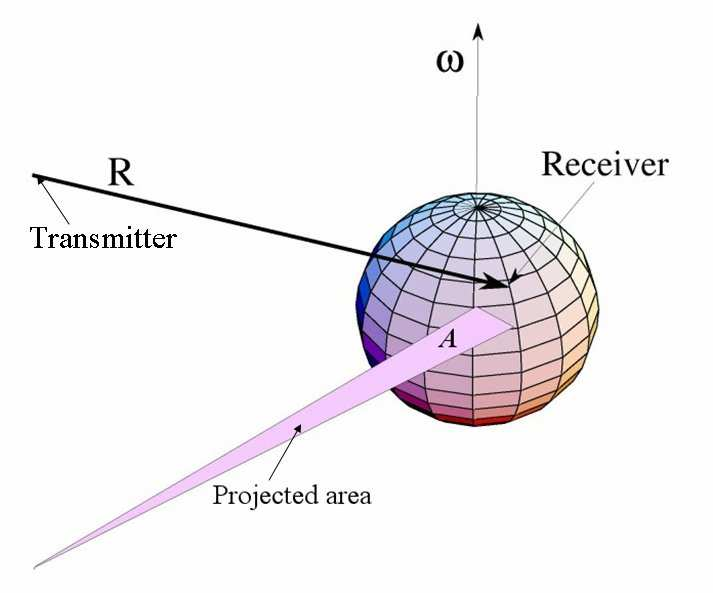
\includegraphics[scale=0.5]{sagnac.png}
\caption{A visualisation of the projection of $A_z$ taken from Ashby's article \cite{ashby2}}
\end{figure}

This transformation produces the metric used in the Sagnac effect \cite{ashby-llr}

\begin{equation} \label{sagnac-metric}
-ds^2 = - \left(1- \frac{\omega_{e}^2 {r'}^2}{c^2}\right)(cdt')^2 + 2 \omega_{e} {r'}^2 d\phi' dt' + (d\sigma')^2
\end{equation}
with $(d\sigma')^2 = (dr')^2 + (r' d \phi')^2 + (dz')^2$. As we recall from chapter two, light travels such that \(ds^2 = 0\) and thus we can form an equation for \(dt'\) which we can solve to give the time of travel for a light ray. If we ignore terms $\frac{\omega_{e}^2 {r'}^2}{c^2} << 1$ we can solve for $dt'$ 
\begin{equation} \label{sagnac-deriv}
	(cdt')^2 - \frac{2\omega_{e} {r'}^2 d\phi' (cdt')}{c} - (d \sigma)^2 = 0
\end{equation}
and thus by solving the quadratic for \(dt'\)
\begin{equation} \label{sagnac-deriv2}
	c dt' = d\sigma + \frac{\omega_{e} {r'}^2 d\phi'}{c} .
\end{equation}

Now, if we integrate \(dt'\) we can obtain the time of travel for light in this spacetime
\begin{equation}
	\int_{\text{path}} dt' = \int_{\text{path}} \frac{d \sigma'}{c} + \frac{2\omega_{e}}{c^2} \int_{\text{path}} d {A'}_{z}
\end{equation}
\noindent where $dA_z$ is the projection of the path taken by an observer on the surface of the earth projected onto a triangular infinitesimal area on a plane through the equator. Thus we observe that the Sagnac effect is dependent on how close you are to the equator: for observers at the pole no such effect would be measured, whereas for observers at the equator this could amount to a discrepancy in measured time from the satellite of up to $\pm 207 $ns. 

\section{Other Relativistic Effects}

There are a few other effects which relativity has on the global positioning system, which do not play as much of a role as compared to the ones above.

These are as follows \cite{ashby-llr, ashby}

\begin{itemize}
	\item Tidal effects on satellite clocks
	\item The non-spherical nature of the earth produces a field which is not quite like the Schwarzschild metric. This produces quadrupole effects on the satellite clocks.
	\item Shapiro delay of the light rays
	\item Relativistic frame dragging due to the rotation of the earth
\end{itemize}